\documentclass[a4paper,10pt]{article}
% portuguese
\usepackage[brazil]{babel}
\usepackage[utf8x]{inputenc}
\usepackage{url}
\usepackage{graphicx}

% Margens: - superior: 2 cm; - inferior: 2 cm; - esquerda: 2 cm, e direita: 2 cm
\usepackage[margin=2cm]{geometry} 

% Fonte: Arial
\usepackage[T1]{fontenc}
\usepackage{uarial}

%opening
\title{Estudo da adequação de plataformas de processamento paralelo de alto 
desempenho para suporte à execução de aplicações de e-Ciência: Relatório
Parcial}
\author{Armstrong Mardilson da Silva Goes}

\begin{document}

\maketitle

\section{Introdução}
% [parallel data processing é util para um bocado de aplicacoes]
% [TODO: revisar esta frase, parece a Veja]
Estamos na era das grandes massas de dados\cite{mapreduce_johnny}.
Empresas como \textit{Facebook}, \textit{Amazon}, \textit{Yahoo} e \textit{Google}
armazenam uma quantidade enorme de dados dos seus clientes e
diariamente geram terabytes em pesquisas e desenvolvimento.
%[TODO: alguma referencia pra isso acima ?]
E-Ciência segue o mesmo caminho. Pesquisas científicas atualmente demandam uma grande quantidade
de recursos computacionais para processar e armazenar os dados gerados em
experimentos. Processar grandes massas de dados é complicado. Em geral é
necessário uma grande quantidade de recursos computacionais para realizar o
processamento.
A utilização de super-computadores é muito dispendiosa. Em vez disso, utilizar processamento 
paralelo é uma opção para tornar pesquisas e desenvolvimento mais baratos. 
Neste contexto encontra-se \textit{MapReduce}.
%[TODO: processamento paralelo e super-computadores não são antagônicos, como parece descrito pelo
%"Em vez disso"]

% [as solucoes atuais tem um custo alto pois assumem infraestruturas dedicadas]
\textit{MapReduce}\cite{Dean04mapreduce:simplified} é um modelo de programação
paralela que descreve a computação em termos de funções \textit{map} e
\textit{reduce}. Este modelo determina que preocupações como transferência de
dados entre máquinas e recuperação de situações de falhas sejam tratadas por
suas implementações, permitindo o desenvolvimento mais fácil de aplicações de
processamento paralelo. Como estas implementações, por exemplo
Hadoop\cite{hadoop_site}, em geral são projetadas para executar em ambientes
dedicados, os custos de aquisição e manutenção de um ambiente deste tipo pode
ser uma barreira para a adoção deste modelo de programação paralela.

%[recursos ociosos tem menor custo]
Uma alternativa de menor custo é a implantação de \textit{MapReduce} em
ambientes oportunistas\cite{Lin:2010:MMO:1851476.1851489}. Um ambiente
oportunista utiliza recursos ociosos, tais como capacidade de armazenamento e
processamento.
%[TODO: acho que a ultima frase nao ajudar muito. melhor seria explicar pro leitor
% porque usar recursos oportunistas apresenta menor custo (tb parece que estamos assumindo que
% ele sabe o que é um "ambiente oportunista" --- que soa estranho, btw).]
%[um requisito é nao atrapalhar a experiencia do usuario]
Uma preocupação comum quando se faz uso de recursos oportunistas é evitar que 
as aplicações prejudiquem a experiência do usuário dono da estação de trabalho.
%[ a tecnica padrao é usar o recurso quando o dono está ausente. o problema é
% que isto é ineficiente]
% TODO add reference to idle resources
Para isso utilizam os recursos das estações de trabalho somente quando estas
estão ociosas. Como consequência, as tarefas são interrompidas quando o usuário
volta à estação de trabalho e trabalho útil é perdido.
%[uma alternative mais a agressiva é ...]
Uma alternativa mais agressiva é executar as tarefas enquanto o usuário estiver
utilizando sua estação de trabalho\cite{W.Strickland:2005:GAT:1078027.1078527}.

%[para adota-la é preciso entender o padrao de intrusividade das aplicacoes. 
% este pesquisa considera a medida deste padrao para Hadoop]
A utilização de \textit{MapReduce} em ambientes oportunistas de forma mais
agressiva pode ser intrusiva, visto que o \textit{MapReduce} vai utilizar
recursos da máquina de modo concorrente com seu usuário. Esta competição por
recursos pode fazer com que a resposta da máquina ao usuário seja mais lenta,
gerando desconforto. No entanto não se sabe se o \textit{MapReduce} é intrusivo
a ponto de tornar inviável sua utilização em ambientes oportunistas. Portanto,
tem-se o problema de determinar o grau de intrusividade do \textit{MapReduce} em
ambientes oportunistas.

\section{Objetivos}

Determinar o grau de intrusividade da utilização de \textit{MapReduce} em
ambientes oportunistas.

\section{Material e Métodos}

\subsection{Métodos}
\label{metodos}
% TODO colocar os outlines antes dos paragrafos

Para medir o grau de intrusividade do \textit{MapReduce}, a metodologia
utilizada baseia-se em reproduzir cargas de trabalho \textit{MapReduce} em
ambientes oportunistas e medir o desconforto dos usuários das máquinas
utilizadas no experimento\cite{Gupta:2004:MUU:1032647.1033307}
\cite{Dinda:2007:UEC:1287050.1287061}.
%[TODO: muita repeticao da palavra "implementacao", so feio]
Para reproduzir as cargas de trabalho uma estratégia possível é utilizar
realmente uma implementação de \textit{MapReduce}, tal como Hadoop, em um
ambiente oportunista. Isto exigiria a instalação de uma implementação da
plataforma no ambiente do experimento bem como lidar com a manutenção e
administração da implementação.

% ao inves de simular, vc esta gerando cargas sinteticas
Em vez disso, a estratégia utilizada foi reproduzir cargas sintéticas do
\textit{MapReduce}. Ao reproduzir estas cargas de trabalho, apesar
de ter de desenvolver uma ferramenta para a reprodução, tem-se uma melhor noção
das características das cargas de trabalho que estão sendo executadas e
realiza-se alterações sobre as cargas de trabalho utilizadas mais facilmente,
podendo assim explorar mais possibilidades.
%[FIXME: está dificil de entender as vantagens de usar uma carga sintetica.
%alem disso é preciso dizer como isto resolve o problema descrito no paragrafo
%anterior]

Hadoop é a implementação de \textit{MapReduce} mais utilizada atualmente, a
exemplo de clusters do
\textit{Facebook}\cite{Borthakur:2011:AHG:1989323.1989438} e da
\textit{Yahoo}\cite{Olston:2011:NCP:1989323.1989439}. Portanto utilizá-lo nos
experimentos de coleta de dados sobre as cargas de trabalho trará resultados
mais próximos da intrusividade do \textit{MapReduce} em ambientes oportunistas reais.
%[TODO, estranho o paragrafo acima. "utilizá-los" ? utilizar quem ?]

% [TODO colocar uma referencia paras as proximas secoes, apontando para a
% parafernalia de instrumentacao]
% na seção tal descrevemos tal, mais detalhes são dados na seção tal
Segundo Chen et al.\cite{Chen:2012:IAP:2367502.2367519}, existe uma
grande variedade de cargas de trabalho de aplicações que
utilizam \textit{MapReduce}. Para abranger uma quantidade satisfatória de cargas
de trabalho a estratégia utilizada foi usar as cargas de trabalho de
\textit{benchmarks} do Hadoop. \textit{Benchmarks} em geral tentam submeter
os sistemas testados a situações de utilização próximas da realidade e podem ser
utilizados para obter cargas de trabalho próximas das reais. 
As cargas de trabalho geradas pelos \textit{benchmarks} utilizados, descritas na
Seção~\ref{resultados_parciais}, foram caracterizadas em termos da utilização
dos
recursos de armazenamento, memória e CPU.

Para a reprodução das cargas de trabalho será desenvolvida uma ferramenta que 
utilizará os recursos de forma a reproduzir a carga na máquina do
usuário e coletará informações sobre o desconforto. Quanto à medição do
desconforto, utilizaremos a estratégia adotada por Gupta et
al.\cite{Gupta:2004:MUU:1032647.1033307}
\cite{Dinda:2007:UEC:1287050.1287061}, que consiste em fornecer uma interface ao
usuário que possibilite a este reportar desconforto durante a reprodução da
carga. Uma vez que tenha ocorrido
uma notificação, a reprodução é interrompida imediatamente para que a
experiência do usuário não seja prejudicada de modo prolongado.

% [estranho, acho que nao entendi direito]
Como o que queremos investigar depende diretamente do usuário, a ferramenta não 
reproduzirá nenhuma carga de trabalho enquanto a máquina estiver ociosa. Entre
as reproduções haverá períodos utilizados como controle. Estes períodos de
controle serão utilizados para coletar dados sobre usuários que relatam
desconforto mesmo quando a ferramenta não estiver rodando a carga de trabalho.
Não realizar esta coleta de forma diferenciada pode levar à confusão entre
desconforto causado pela reprodução das cargas de trabalho e desconforto
causado por exemplo pelas próprias aplicações utilizadas pelo usuário.
A duração desses períodos será variável para impedir que o usuário detecte padrões
na execução da ferramenta.

% TODO suponha dois usuário que participam do experimento: usuário A e usuário B
% usuário A utiliza programas que consomem uma grande quantidade de recursos
% computacionais, enquanto que usuário B utiliza programas que consomem poucos
% recursos computacionais. É mais provável que a reprodução de cargas de
% trabalho na máquina do usuário A cause desconforto do que a reprodução na
% máquina do usuário B. Portanto, podemos, para a mesma carga de trabalho, obter
% resultados diferentes, sendo que esta variação nos resultados não é imposta
% pela diferença de sensibilidade dos usuários à perda de desempenho, e sim
% pela diferença das suas atividades quando a carga de trabalho foi reproduzida.
% portanto, ao coletar também o consumo de recursos computacionais utilizados
% pelo usuário, podemos ter certeza de que o desconforto foi gerado pela carga
% de trabalho ou não.

A atividade do usuário pode contribuir para o incômodo durante a reprodução das
cargas de trabalho. Caso o usuário realize tarefas que utilizem grandes
quantidades de recursos computacionais a reprodução das cargas de trabalho,
devido à maior competição por recursos, provavelmente gerará mais desconforto do
que se o usuário realizar tarefas menos exigentes. Portanto, coletaremos também
a utilização de recursos tais como CPU, memória e disco pelo usuário para
descobrir os níveis de utilização das máquinas quando o desconforto for
reportado.

A Seção \ref{material} expõe mais detalhes sobre a arquitetura da ferramenta.

\subsection{Material}
\label{material}

% [TODO acho que é preciso manter um inventario, ou ate mesmo, rodar um
% benchmark para quantificar
% a capacidade de processamento dos desktops]
% [TODO porque nao um experimento controlado?]
Para a execução do experimento, serão utilizadas as estações de trabalho do
Laboratório de Sistemas Distribuídos da Universidade Federal de Campina Grande.
Os usuários destas estações são em sua maioria pesquisadores da área de Ciência 
da Computação e sistemas distribuídos. Estes em geral utilizam suas máquinas
para realização de pequenos experimentos locais, acesso à internet, edição de
documentos e desenvolvimento de programas de computador para seus experimentos. 
A maior parte das máquinas em geral utilizam sistemas operacionais baseados em
Linux, portanto o foco no desenvolvimento da ferramenta citada na seção anterior
é seu funcionamento neste tipo de sistema operacional. Em termos de configuração
das máquinas o Laboratório de Sistemas Distribuídos é um ambiente heterogêneo.
%[TODO: qual a importancia disto que está escrito na ultima frase]

A ferramenta que será desenvolvida, ilustrada pela Figura
\ref{tools_architecture}, será composta pelos seguintes módulos:\newline
\newline
\textbf{Reprodutor de cargas}: responsável por reproduzir na máquina do usuário
as cargas de trabalho coletadas na primeira etapa do projeto.\newline
\textbf{Controlador de Reprodução}: coordenará as ações do Reprodutor de Cargas,
para que este aja somente nos momentos adequados. A Seção~\ref{metodos} descreve
as situações nas quais o Controlador de Reprodução ordenará ao Reprodutor de
Cargas que inicie as reproduções.\newline
\textbf{Coletor de Resultados}: coletará e organizará os resultados dos
experimentos. Entre os dados coletados estão o tempo transcorrido entre o início
da reprodução e o relato do desconforto e a carga de trabalho que possivelmente
causou o desconforto.\newline
\textbf{Interface}: permitirá ao usuário reportar desconforto. Esta
interface será composta por um ícone visível na área de trabalho. Ao
clicar no ícone, a reprodução das cargas sintéticas será interrompida.\newline
%[FIXME: trocar "Interface" por "Interface de xpto", inventar um xpto bacana]

\begin{figure}[htp]
 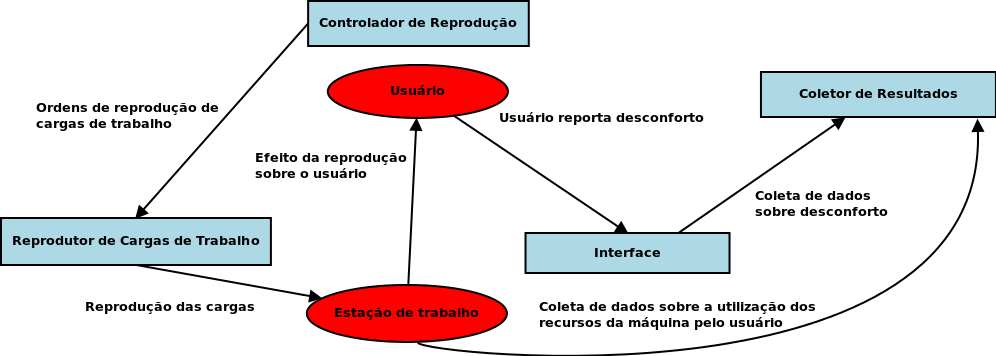
\includegraphics[width=17cm]{arquitetura_ferramenta.png}
 \caption{Arquitetura da ferramenta utilizada para a medição da intrusividade.
Os módulos da ferramenta são apresentados como retângulos azuis e outros
componentes são apresentados como elipses vermelhas. As setas representam as
interações entre os elementos e o fluxo de informações no sistema.}
 \label{tools_architecture}
\end{figure}

\section{Resultados parciais}
\label{resultados_parciais}

Os primeiros meses do projeto foram destinados à aquisição de conhecimento
sobre medição de intrusividade em sistemas computacionais, sobre
\textit{MapReduce} e suas implementações e à coleta da informação sobre cargas de
trabalho \textit{MapReduce}.
%[TODO: uma opcao é escrever um resumo do que será visto nas proximas subsecoes]

\subsection{Coleta de informação sobre cargas de trabalho}

\subsubsection{Ambiente de execução}

No Hadoop, implementação otimizada para ambientes homogêneos, cada
máquina recebe aproximadamente a mesma quantidade de dados para processar.
Consequentemente, para um conjunto de máquinas semelhantes os resultados do
consumo de recursos devem ser semelhantes. Portanto, só é necessário realizar
medições em uma máquina. A medição realizada levou em conta o raciocínio
descrito, executando o Hadoop em apenas uma máquina.
%[TODO: achei um pouco confusa esta explicacao, parece dar a entender que a carga
%imposta pelo hadoop seria diferente em maquinas diferentes]

% TODO descobrir a quantidade de slots utilizados
A versão do Hadoop utilizada para rodar os \textit{benchmarks} foi a $1.1.1$.
Quanto à sua configuração foi utilizada a padrão do Hadoop para todas as
características.

% [TODO porque esta maquina ?]
% [TODO mais configuracoes de hw ... disk ... ]
% [TODO configuracoes das aplicacoes sao importantes ? java etc ?
A configuração da máquina utilizada é apresentada na Tabela
\ref{machine_configuration}.

\begin{table}[htp]
   \centering
   \caption{Configuração da máquina} 
   \label{machine_configuration}
   \begin{tabular}{|c|c|}
      \hline
      CPU & Intel Core 2 Duo 1998 MHz \\
      \hline
      Memória principal & 2 GB \\
      \hline
      Memória Cache & 8 MB \\
      \hline
      Sistema Operacional & Ubuntu 10.04.4 LTS com kernel Linux 2.6.32-28 \\
      \hline
   \end{tabular}
\end{table}

\subsubsection{Código de instrumentação}
A utilização de memória e CPU foi coletada a partir de scripts. Para coletar
%[FIXME, dizer que foi coletada a partir de scripts nao ajuda. tenha em mente que
% o objetivo é permitir que alguem reproduza seu trabalho]
informações sobre utilização de disco, instrumentamos o kernel utilizando a
ferramenta SystemTap\cite{systemtap_site}. Esta ferramenta guarda
registros das chamadas ao sistema determinadas. No experimento, configuramos a
ferramenta para guardar registros de escritas, leituras e operações
\textit{seek}.
%[FIXME: qual a razão de escolher deste subconjunto ?]

\subsubsection{\textit{Benchmarks} utilizados}

Procuramos escolher \textit{benchmarks} a partir dos quais pudéssemos coletar
uma quantidade satisfatória de dados sobre cargas de trabalho
\textit{MapReduce}. Os três \textit{benchmarks} escolhidos, que reproduzem
cargas de trabalho particulares e dos quais coletamos a utilização de CPU,
memória e disco são:
\newline \newline
\textbf{MRBench\cite{benchmarks}\cite{Kim:2008:MBM:1491261.1491574}}: utilizado
para medir o desempenho do \textit{cluster} ao executar \textit{jobs} baseados 
em operações sobre bancos de dados. Ele se concentra em verificar o
desempenho da implementação de \textit{MapReduce} quando executados
\textit{jobs} de curta duração.\newline
\textbf{TestDFSIO\cite{benchmarks}}: Utilizado para medir o desempenho do
\textit{cluster} em termos de IO e o sistema de arquivos utilizado pelo
\textit{MapReduce}. Neste caso utilizamos o sistema de arquivos do Hadoop, o
HDFS (Hadoop Distributed File System). A carga de trabalho gerada por
este \textit{benchmark} é basicamente IO \textit{bound}.\newline
\textbf{Terasort\cite{benchmarks}}: Tem como objetivo ordenar uma quantidade de
dados determinada. É utilizado para verificar o desempenho do sistema como um
todo e para comparar poder de processamento de \textit{clusters}. A
carga de trabalho gerada por este \textit{benchmark}
espera-se que seja CPU \textit{bound}\newline
%[FIXME: cluster ? que cluster ? a explicao nestes bullets está muito confusa]

Cada \textit{benchmark} pode ser configurado quanto à quantidade de dados
processada ou de \textit{jobs} executados. As configurações utilizadas para o
TestDFSIO são descritas na tabela \ref{configuration_testdfsio}. Quanto ao
MRBench executamos o \textit{benchmark} com o valor 10 para o parâmetro
Quantidade de \textit{jobs}, e quanto ao Terasort utilizamos o valor 1000000
para o parâmetro Número de linhas de 100 bytes.

\begin{table}[htp]
  \centering
  \caption{Configuração TestDFSIO}
  \label{configuration_testdfsio}
  \begin{tabular}{|c|c|c|}
      \hline
      Configuração & Quantidade de arquivos & Tamanho dos arquivos (em MB) \\
      \hline
      \hline
      1 & 1 & 100 \\
      \hline
      2 & 100 & 1 \\
      \hline
  \end{tabular}
\end{table}

As configurações escolhidas para o TestDFSIO visaram abranger uma quantidade
maior de cargas de trabalho. Note que as duas configurações retratam cenários
opostos: aplicações que manipulam poucos arquivos grandes e aplicações
que manipulam muitos arquivos pequenos.
 
O parâmetro mais importante para o MRBench é a quantidade de \textit{jobs} que
serão executados. Em uma execução do \textit{benchmark} em um sistema com apenas
uma máquina e utilizando Hadoop, que fixa o número de \textit{mappers} e
\textit{reducers} de cada nó do sistema, a variação do número de \textit{jobs}
não resulta em variações significativas na carga de trabalho produzida.

Quanto ao Terasort, o parâmetro principal é a quantidade de dados que serão
ordenados. No Hadoop a quantidade de dados enviados a cada \textit{mapper} e
\textit{reducer} é fixa. Portanto, variar a quantidade de dados utilizados como
entrada para o \textit{job} não resulta em variação na quantidade de dados
processada em cada máquina, e, consequentemente, não gera variações
significativas na carga de trabalho produzida.

A partir das ideias descritas acima decidimos executar o MRBench e o Terasort
com apenas uma configuração.

\section{Planejamento}

\subsection{\textbf{Atividades a serem realizadas até o fim do projeto}}

\begin{description}
  \item[$\bullet$ Desenvolvimento da ferramenta de medição de intrusividade] 
  \item[$\bullet$ Instalação da ferramenta no ambiente do experimento]
  \item[$\bullet$ Execução do experimento e coleta de resultados]
  \item[$\bullet$ Escrita do relatório final]
\end{description}

\subsection{\textbf{Gerência do Tempo}}

\textbf{Tempo disponível: 5 meses (Março, Abril, Maio, Junho e Julho)}\newline

Informações sobre como o tempo disponível será distribuído entre as atividades
estão disponíveis na Tabela \ref{time_management}

\begin{table}[htp]
  \centering
  \caption{Cronograma}
  \label{time_management}
  \begin{tabular}{|c|c|c|c|c|c|}
    \hline
      Atividade & Março & Abril & Maio & Junho & Julho \\
    \hline
    \hline
      Desenvolvimento da ferramenta & X & X & & & \\ 
    \hline
      Instalação da ferramenta & &  & X & & \\
    \hline
      Execução do experimento & & & X & X & \\
    \hline
      Escrita do relatório final & X & X & X & X & X \\
    \hline
  \end{tabular}
\end{table}

\null
\vfill
\newpage
\bibliography{partial_report}
\bibliographystyle{acm}

\newpage
\null
\vfill
Assinatura do Bolsista:  \underline{\hspace{12cm}}
\newline
Assinatura do Orientador:  \underline{\hspace{12cm}}
\newline
Campina Grande, \underline{\hspace{1cm}} / \underline{\hspace{1cm}} /
\underline{\hspace{1cm}}\newline

\end{document}
